\subsection{Convergencia}
\label{subsec:exp3}
\begin{LaTeXdescription}
    \item[Objetivo] Estudiar como se comporta la convergencia en funci\'on de
        el factor de navegaci\'on $\alpha$.

    \item[Proposici\'on] PageRank propone una soluci\'on donde se observa a un
        conjunto de p\'aginas web como un grafo dirigido. Luego pasa este modelo
        a uno  matem\'atico, utilizando una matriz para computar una soluci\'on.
        Esta matriz, por construcci\'on, termina representando a un grafo
        completo (el grafo original no necesariamente lo era), y los valores del
        mismo dependen principalmente de 2 variables: $\epsilon$ y $\alpha$
        (algoritmo \ref{alg:power_method2}, p\'agina \pageref{alg:power_method2}
        y ecuaci\'on \ref{eq:M_def}, p\'agina \pageref{eq:M_def}). Si se observa
        el algoritmo, se ver\'a que claramente modificar el $\epsilon$ tendr\'a
        como resultado hacer que cada corrida converja en m\'as o menos
        iteraciones, ya que el criterio de parada depende de \'el. As\'i pues,
        no vemos como algo rico experimentar con este valor. En cambio, $\alpha$
        es una variable que modifica en gran medida a nuestra matriz $M$, con lo
        cual es dificil saber cual ser\'a su injerencia en la convergencia (en
        principio). El objetivo, entonces, es ver como $\alpha$ afecta al
        m\'etodo matem\'atico iterativo de la potencia en cuanto a su
        convergencia.

    \item[M\'etodo de Experimentaci\'on] Tomaremos 3 instancias de grafos de
        conectividad de p\'aginas web de tama\~no mediano-grande, obtenidas en
        \url{http://snap.stanford.edu/data/\#web}. Luego, correremos el
        algoritmo de PageRank para $\alpha=0.0$; $0.1$; $0.2$; $\dots$; $0.9$ y $\epsilon$
        fijo en $0.00001$

    \item[Resultados, an\'alisis y discusi\'on]
    En el gráfico \ref{subfig:exp3_comp} se exponen la cantidad de iteraciones necesarias hasta converger a medida que el parámetro $\alpha$ crece, para las 3 instancias, el comportamiento observado es el mismo, puede observarse que aunque con valores numéricos diferentes, las curvas pertenecen a la misma familia de funciones.\\

    Respecto a la velocidad de convergencia, exponemos los resultados de una sola instancia ya que para las 3 instancias los resultados son similares: Como puede observarse en el gráfico \ref{subfig:exp3_diff}, a medida que el factor de navegacion $ \alpha $ crece, la velocidad de convergencia disminuye, es decir, la distancia manhattan entre iteraciones se acerca \texttt{mas rápido} al umbral de corte del algoritmo en términos de cantidad de iteraciones.\\

    Se nos ocurre conjeturar que en un contexto de una cadena de markov y el navegante aleatorio, un $\alpha$ pequeño nos genera una cadena de markov mas equiprobable y dado que el método de la potencia comienza inicialmente con el vector equiprobable, le toma pocas iteraciones converger. A medida que $\alpha$ aumenta, el grafo generado denota más la navegación estricta por los links entre los sitios con menor probabilidad de teletransportación. Es decir, a mayor $\alpha$, el grafo se parece mas al grafo de conectividad original no adulterado. Este grafo original no necesariamente representa un grafo fuertemente conexo, una de las condiciones necesarias para asegurar convergencia del método de la potencia en el contexto de este problema, con lo cual el método de la potencia inicia sus iteraciones con una \texttt{seguridad de convergencia más débil}.
\end{LaTeXdescription}

\begin{figure}[!h]
    \centering
    \subfloat[][Iteraciones hasta Converger en funci\'on de $\alpha$]{
        \label{subfig:exp3_comp}
        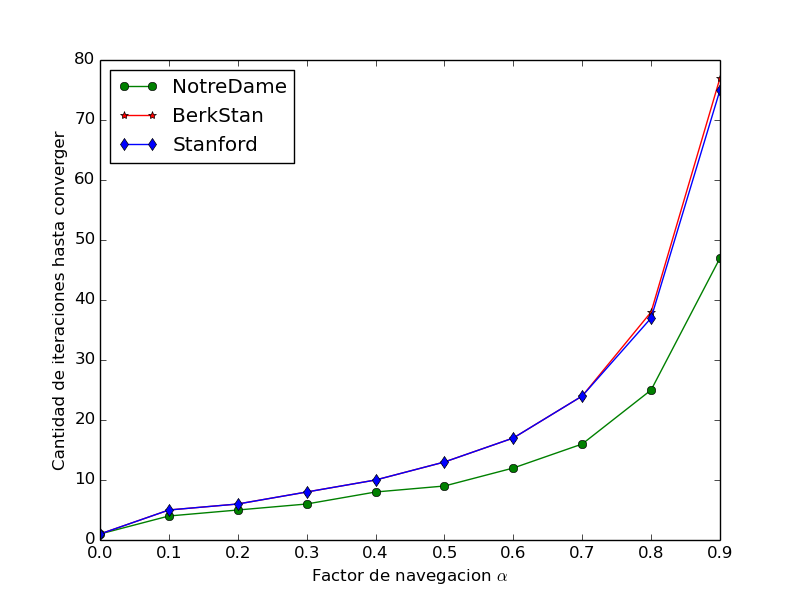
\includegraphics[width=.5\textwidth]{exp3_iteraciones_funcion_alpha.png}
    }
    \subfloat[][Velocidad de convergencia en funci\'on de $\alpha$]{
        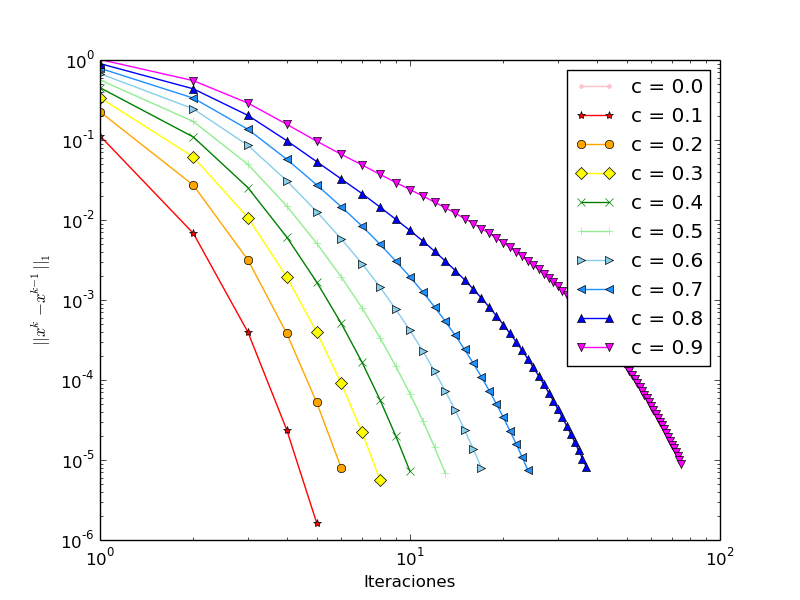
\includegraphics[width=.5\textwidth]{exp3_diff_funcion_iteraciones_standford.png}
        \label{subfig:exp3_diff}
    }
    \caption{An\'alisis de Convergencia en funci\'on de $\alpha$}
\end{figure}


%\label{[fig,subfig,itm,alg,tbl,eq]:nombre_a_eleccion}de ahí los prefijos que no se entienden por ahí son: itm (itemize), alg(algoritmo), tbl(tabla/cuadro), eq (ecuacion)